\documentclass{tufte-handout}
\usepackage{amsmath,amsthm}
\usepackage{fancyvrb}
\fvset{tabsize = 4}
\fvset{fontsize = \small}

\usepackage{pgfplots}
%\pgfplotsset{width=\textwidth,compat=1.5.1}

\newtheorem{claim}{Claim}[section]
\title{\sf Rainbow Perfect Matchings}
\author{Mats Rydberg \& Martin Larsson}

\begin{document}
\maketitle

\section{Algorithm}
\begin{enumerate}
\item Fix prime $p \gg n$ \sidenote{In our case, we selected $p = 32749$.}
\item For each colour $C \in [n]$
\subitem Construct $n \ast n$ matrix $m_C$
\subitem For each $uv \in E$ with $ c(uv) = C$
\subsubitem Pick random integer $r \in (0,p]$
\subsubitem Set $m_C[u,v] = r$
\item Set $B = \sum_{i = 0}^{n-1}m_i$
\item Compute $d_B =$ det$(B)$ mod $p$
\item If $d_B = 0$ return ''no''
\item Else set $sum = 0$
\item For each $X \subset [n]$
\subitem Initialize $M = \mathbf{0}$ \sidenote{$\mathbf{0}$ is the $n \ast n$ all-zeroes matrix.}
\subitem For each $C \in X$
\subsubitem Set $M = M + m_C$
\subitem Set $sum = sum + (-1)^{n-|X|-1} \cdot$ det$(M)$ mod $p$
\item If $d_B - sum = 0$ return ''no'' else return ''yes''
\end{enumerate}

\noindent Our algorithm modifies the given Algorithmic Piece 1 on step 2, by creating $n$ matrices, one for each colour. But in step 3 we combine them into the biadjacency matrix $B$ (called $A_G$ in the assignment) and do the same end condition for its determinant.

For Algorithmic Piece 2, we have modified the pseudo code to be defined via matrix sums instead. We construct the biadjacency matrix for the current set of colours by simple addition, and compute the determinant for every such matrix. We are not including det($B$) in $sum$, so to get the signs right we subtract an extra $1$ in the exponent for $-1$.\sidenote{Another way to fix this would be to compute $d_B + sum$ in step 7 of the algorithm, but we thought this was cleaner.} This is really just an optimization, as we could remove steps 3 and 4 and have Algorithmic Piece 2 more or less intact. Our algorithm is faster for ''no''-instances, however. With this change in mind, the logic is the same as in the assignment for why a non-rainbow perfect matching will eliminate itself in the calculation of $sum$.
\newpage





\section{Running Time}
In our calculations, we define the basic, constant-time operations to be scalar additions and scalar multiplications. Any other operation we assume to take no time.

We are only interested in a running time bound with respect to $n$, hence we assume a worst-case $m = n^2$, and do not include $m$ in our $O$-notation.

Step by step, we pay as follows:

\begin{enumerate}
\item No time.
\item $n$ repetitions of
\subitem No time.
\subitem Worst case $n$ edges of colour $C$ from all $n$ nodes $\Rightarrow T(n) = n^2$ repetitions of
\subsubitem No time.
\subsubitem No time.
\item $T(n) = n^3$ additions $\Rightarrow T(n) = n^3$
\item $T(n) = \frac{2}{3}\cdot n^3 \Rightarrow T(n) =\frac{2}{3} n^3$ \sidenote{Knowing our determinant calculation implements Gaussian elimination, this is the number of operations required. Normally, this would have exponential bit complexity, but our calculations are made modulus $p$, and are thus constant in bit complexity \cite{wikiGauss}.}
\item No time.
\item No time.
\item There are $2^n$ subsets to a set of $n$ elements $\Rightarrow T(n) = 2^n - 2$ (the empty set and the full set) repetitions of
\subitem No time.
\subitem On average for each $X$, $T(n) = \frac{1}{2} n$ \sidenote{This follows from how frequent a given size of an element in the power set of $[n]$ is \cite{powerset}.} repetitions of
\subsubitem $n^2$ additions $\Rightarrow T(n) = n^2$
\subitem $1$ addtition, worst case $n - 2$ multiplications of $-1$, $1$ multiplication and $T(n) = \frac{2}{3}n^3$ cost for determinant calculation gives $T(n) = 1 + (n - 2) + 1 + \frac{2}{3}n^3 = \frac{2}{3}n^3 + n$
\item $1$ addtition $\Rightarrow T(n) = 1$
\end{enumerate}

This results in final running time of

$$
T(n) = 0 + n(0 + n^2(0 + 0)) + n^3 + \frac{2}{3}n^3 + 0 + 0 + (2^n - 2)(0 + \frac{1}{2}n (n^2) + \frac{2}{3}n^3 + n) + 1
$$

$$
= \frac{5}{3}n^3 + (2^n - 2)(\frac{7}{6}n^3 + n) + 1
$$

$$
= \frac{5}{3}n^3 + 1 - \frac{7}{3}n^3 - 2n + 2^n(\frac{7}{6}n^3 + n)
$$

$$
= 1 - 2n - \frac{2}{3}n^3 + 2^n(\frac{7}{6}n^3 + n)
$$

The dominant factor here is, as expected, exponential in $n$. Thus we do have $O^*(2^n)$. We could also present a running time bound of $O(n^3\cdot2^n)$, in which we consider all factors with an exponential in $n$ relevant, and take the largest-degree polynomial of this factor as our bound.

The exponential $2^n$ factor come from the fact that we are traversing the power set of an $n$-sized set. The plynomial $n^3$ factor comes from our determinant calculation, which runs this fast. Thus, the $O(n^3\cdot2^n)$ really summarizes our algorithm in a nice way; we do calculate a determinant for a matrix corresponding to every element of the power set of $[n]$.

\newpage
\section{Failure bound}



\begin{marginfigure}
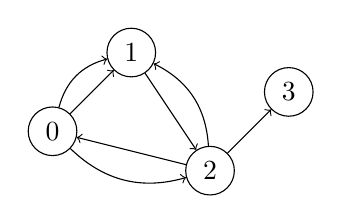
\begin{tikzpicture}
\node (0) [draw,circle] at (0,0) {0};
\node (1) [draw,circle] at (1,1) {1};
\node (2) [draw,circle] at (2,-.5) {2};
\node (3) [draw,circle] at (3,.5) {3};
\draw [->] (0) to [bend left] (1);
\draw [->] (0) to  (1);
\draw [->] (0) to [bend right] (2);
\draw [->] (1) to  (2);
\draw [->] (2) to  (0);
\draw [->] (2) to [bend right] (1);
\draw [->] (2) to (3);
\end{tikzpicture}
\caption{A directed multigraph.}
\end{marginfigure}

\section{Analysis}

\subsection{Lol}

The files are in the data directory are:
\begin{quotation}
\begin{description}
\item[three.txt] The 4-vertex graph from Fig.~1.
\end{description}
\end{quotation}

\section{Report part maybe}

\subsection{Transition probabilities}

The transition matrix for the graph described in three.txt
is\sidenote{Fill in the right values. Set $\alpha=\frac{85}{100}$.}
\begin{equation*}
P = 
\left(
\begin{array}{cccc}
1 & 6 & \pi & 1\\
1 & 1/e & -2  & \cdots\\
1 & 1 & 0 \\
\vdots
\end{array}
\right)\,,
\end{equation*}

\noindent text is text is text is text

\medskip
\begin{fullwidth}
\small
\begin{tabular}{lcccccccccc}
three.txt & 2 (36.6\%) & 1 (27.5\%) & 0 (18.4\%) & 3 (17.3\%) \\
tiny.txt & [\ldots] &\\
medium.txt &\\
wikipedia.txt & \\
p2p-Gnutella08-mod.txt &
\end{tabular}
\end{fullwidth}

\appendix

\section{Implementation}
This is our implementation of our Perfect Rainbow Matching algorithm. It is only sparsely commented, but we expect its behaviour to be fairly straight-forward. We have tried to follow our pseudo-code verbatim, putting aside Java programming practices to some extent.
\VerbatimInput{Main.java}

\begin{thebibliography}{9}
\bibitem{powerset} Wikipedia, the Free Encyclopedia, \emph{Power set},  \url{http://en.wikipedia.org/wiki/Power_set#Relation_to_binomial_theorem}, 10 October 2012 05:20
\bibitem{wikiGauss} Wikipedia, the Free Encyclopedia, \emph{Gaussian elimination}, \url{http://en.wikipedia.org/wiki/Gaussian_elimination#Analysis}, 29 September 2012 03:39
\end{thebibliography}


\end{document}
